\section{Implementación}
\label{sec:implementacion}

La materialización del sistema GESCOMPH se ha llevado a cabo utilizando el marco de trabajo \textbf{.NET 8}, aprovechando sus mejoras de rendimiento (LTS) y sus capacidades nativas para la inyección de dependencias. La arquitectura elegida no es un monolito convencional, sino un \textbf{Monolito Modular}. Esta distinción es crucial: mientras que un monolito tradicional tiende a convertirse en una "gran bola de lodo" con el tiempo, nuestra implementación utiliza barreras físicas estrictas para emular la separación de intereses de los microservicios, pero sin la complejidad operativa ni la latencia de red que estos conllevan, una decisión respaldada por los análisis de rendimiento de \cite{monolithic_vs_microservices_blinowski}.

\begin{figure}[H]
    \centering
    \resizebox{0.5\textwidth}{!}{\begin{tikzpicture}[
    every node/.append style={font=\small},
    node distance=3cm and 3cm, % Aumentado para evitar solapamiento
    auto,
    block/.style={rectangle, draw=black, thick, fill=white, text width=3.5cm, align=center, minimum height=1.5cm, rounded corners},
    container/.style={rectangle, draw=black!60, dashed, fill=gray!5, inner sep=0.5cm, rounded corners},
    cloud/.style={cloud, draw=black, thick, fill=blue!5, aspect=2, minimum width=3cm, minimum height=1.5cm}
]
    % Nodos
    \node[block, fill=green!10] (client) {\textbf{Cliente Web/Móvil} \\ (Browser / App)};
    
    % Contenedor Docker
    \node[block, right=of client, fill=blue!10] (api) {\textbf{GESCOMPH API} \\ (.NET 8 Container)};
    \node[block, below=of api, fill=orange!10] (db) {\textbf{SQL Server} \\ (Database Container)};
    
    % Servicios Externos
    \node[block, right=of api, fill=red!10] (external) {\textbf{MercadoPago} \\ (Pasarela de Pagos)};

    % Contenedor lógico (Docker Host)
    \begin{scope}[on background layer]
        \node[container, fit=(api) (db), label=above:\textbf{Docker Host / Cloud Infrastructure}] (host) {};
    \end{scope}

    % Flechas
    \draw[thick, <->, >=stealth] (client) -- node[above, font=\scriptsize] {HTTPS / JWT} (api);
    \draw[thick, <->, >=stealth] (api) -- node[right, font=\scriptsize] {EF Core / TCP} (db);
    \draw[thick, <->, >=stealth] (api) -- node[above, font=\scriptsize] {REST API} (external);

\end{tikzpicture}
}
    \caption{Arquitectura de Alto Nivel del Sistema GESCOMPH. Se muestra el despliegue en contenedores, la comunicación con la base de datos y la integración con servicios externos.}
    \label{fig:arquitectura_alto_nivel}
\end{figure}

\subsection{Arquitectura Física y Segregación de Proyectos}

Para garantizar que la arquitectura teórica se respete en el código, la solución se ha fragmentado físicamente en cuatro proyectos de biblioteca de clases (\texttt{.csproj}) independientes. Esta separación impide referencias circulares y obliga a los desarrolladores a seguir el flujo de dependencia unidireccional.

\begin{figure}[H]
    \centering
    \resizebox{0.5\textwidth}{!}{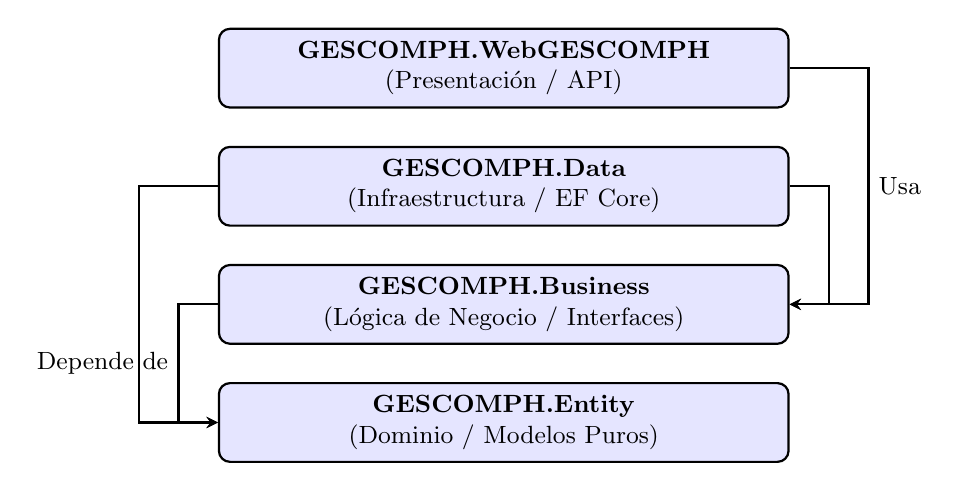
\begin{tikzpicture}[
    every node/.append style={font=\small},
    node distance=1.5cm, 
    auto,
    project/.style={rectangle, draw=black, thick, fill=blue!10, text width=7cm, align=center, minimum height=1cm, rounded corners},
    arrow/.style={thick, ->, >=stealth}
]
    % Nodos representando los proyectos
    \node[project] (web) {\textbf{GESCOMPH.WebGESCOMPH} \\ (Presentación / API)};
    \node[project, below of=web] (data) {\textbf{GESCOMPH.Data} \\ (Infraestructura / EF Core)};
    \node[project, below of=data] (business) {\textbf{GESCOMPH.Business} \\ (Lógica de Negocio / Interfaces)};
    \node[project, below of=business] (entity) {\textbf{GESCOMPH.Entity} \\ (Dominio / Modelos Puros)};

    % Flechas de dependencia
    \draw[arrow] (web.east) -- ++(1cm,0) |- (business.east) node[pos=0.25, right] {Usa};
    \draw[arrow] (data.east) -- ++(0.5cm,0) |- (business.east);
    \draw[arrow] (business.west) -- ++(-0.5cm,0) |- (entity.west) node[pos=0.25, left] {Depende de};
    \draw[arrow] (data.west) -- ++(-1cm,0) |- (entity.west);
    
    % Nota: Web también usa Data para inyección, pero arquitectónicamente pasa por Business
    % Simplificamos para claridad del diagrama
\end{tikzpicture}
}
    \caption{Diagrama de Dependencias Físicas de la Solución. Las flechas indican la dirección de la referencia entre proyectos, garantizando un núcleo (Entity) libre de dependencias externas.}
    \label{fig:arquitectura_fisica}
\end{figure}

\begin{itemize}
    \item \textbf{Capa de Dominio (\texttt{GESCOMPH.Entity}):} Básicamente, aquí vive el corazón del sistema. Tenemos una carpeta \texttt{Domain/Models/Implements} donde pusimos las clases principales: \texttt{Contract.cs}, \texttt{Clause.cs} y \texttt{Establishment.cs}. Son POCO (\textit{Plain Old CLR Objects}), lo que en cristiano significa que son clases normales y corrientes, sin heredar de nada raro. ¿Por qué? Porque queríamos que la lógica de negocio no dependiera de si usamos SQL Server, PostgreSQL o lo que sea. También metimos algunas carpetas para \texttt{Enums} y \texttt{DTOs}, que son los objetos que pasamos de un lado a otro cuando necesitamos compartir información.

    \item \textbf{Capa de Lógica de Negocio (\texttt{GESCOMPH.Business}):} Si la capa anterior es el corazón, esta es el cerebro. La organización es simple: tenemos una carpeta de \texttt{Interfaces} donde decimos "esto es lo que necesito", y otra de \texttt{Services} donde decimos "así es como lo hago". Tomemos \texttt{ContractService.cs} como ejemplo. Este archivo tiene todo el código para validar contratos nuevos, revisar que cumplan las reglas, etc. Pero no toca la base de datos directamente. Para eso usa \texttt{IContractRepository}, que es solo una interfaz. Ah, y hay algo que vale mencionar: \texttt{CustomJWT/TokenBusiness.cs}. Este archivo se encarga de crear los tokens de autenticación. Lo separamos así para que los controladores no se preocupen por cómo se generan los tokens, solo los piden y ya.

\begin{lstlisting}[style=csharp, caption={Generación de Tokens JWT (TokenBusiness.cs). La lógica de seguridad está centralizada y desacoplada de la capa web.}, label={lst:token_business}]
public async Task<TokenResponseDto> GenerateTokensAsync(UserAuthDto user)
{
    var accessToken = BuildAccessToken(user);
    var refreshPlain = TokenHelpers.GenerateSecureRandomUrlToken(64);
    
    // Hashing del refresh token antes de persistir
    var refreshHash = HashRefreshToken(refreshPlain);

    await _refreshRepo.AddAsync(new RefreshToken
    {
        UserId = user.Id,
        TokenHash = refreshHash,
        ExpiresAt = DateTime.UtcNow.AddDays(_jwtSettings.RefreshTokenExpirationDays)
    });

    return new TokenResponseDto
    {
        AccessToken = accessToken,
        RefreshToken = refreshPlain,
        ExpiresAt = DateTime.UtcNow.AddMinutes(_jwtSettings.AccessTokenExpirationMinutes)
    };
}
\end{lstlisting}

    \item \textbf{Capa de Infraestructura de Datos (\texttt{GESCOMPH.Data}):} Este proyecto es el único que tiene permiso para "hablar" con la base de datos SQL Server. En su interior, la carpeta \texttt{Services} (que actúa como implementación de repositorios) contiene clases como \texttt{ContractRepository.cs} y \texttt{EstablishmentsRepository.cs}. Estas clases utilizan \textbf{Entity Framework Core} para traducir las operaciones de negocio en consultas SQL optimizadas. La segregación es tal que el \texttt{DbContext} y las migraciones están confinados aquí, protegiendo al resto del sistema de cambios en el esquema de la base de datos.

\subsection{Seguridad Profunda: Estrategia de Tokens}
La seguridad en GESCOMPH no se limita a un simple login. Implementamos un esquema robusto de autenticación basado en **JWT (JSON Web Tokens)** con rotación de **Refresh Tokens**, diseñado para mitigar el robo de sesiones sin comprometer la experiencia del usuario.

El flujo de autenticación sigue estos pasos estrictos:
\begin{enumerate}
    \item El usuario se autentica y recibe un \texttt{AccessToken} de vida corta (15 minutos) y un \texttt{RefreshToken} de vida larga (7 días).
    \item El \texttt{RefreshToken} se almacena en la base de datos como un hash criptográfico (SHA-256), nunca en texto plano, para prevenir fugas si la base de datos es comprometida.
    \item Cuando el \texttt{AccessToken} expira, el cliente envía el \texttt{RefreshToken}. El sistema valida el hash, verifica que no haya sido revocado y emite un nuevo par de tokens.
    \item **Rotación:** Cada vez que se usa un \texttt{RefreshToken}, este se invalida y se reemplaza por uno nuevo (Family of Tokens). Si un atacante intenta reusar un token antiguo, el sistema detecta la anomalía e invalida toda la cadena de confianza, forzando al usuario legítimo a loguearse de nuevo.
\end{enumerate}

\begin{lstlisting}[style=csharp, caption={Lógica de Generación de Tokens Seguros. Se observa el hashing del Refresh Token antes de la persistencia.}, label={lst:token_logic}]
public async Task<TokenResponseDto> GenerateTokensAsync(UserAuthDto user)
{
    // 1. Generar Access Token (Stateless)
    var accessToken = BuildAccessToken(user);
    
    // 2. Generar Refresh Token (Opaque)
    var refreshPlain = TokenHelpers.GenerateSecureRandomUrlToken(64);
    
    // 3. Hashear para almacenamiento seguro
    var refreshHash = HashRefreshToken(refreshPlain);

    // 4. Persistir con expiración y vinculación al usuario
    await _refreshRepo.AddAsync(new RefreshToken
    {
        UserId = user.Id,
        TokenHash = refreshHash,
        ExpiresAt = DateTime.UtcNow.AddDays(7),
        IsRevoked = false
    });

    return new TokenResponseDto(accessToken, refreshPlain);
}
\end{lstlisting}

\begin{lstlisting}[style=csharp, caption={Implementación del Repositorio de Contratos (ContractRepository.cs). Se observa el uso de EF Core para consultas optimizadas y transacciones implícitas.}, label={lst:contract_repo}]
public class ContractRepository : DataGeneric<Contract>, IContractRepository
{
    public ContractRepository(ApplicationDbContext context) : base(context) { }

    private IQueryable<Contract> GetContractFullQuery()
    {
        return _dbSet
            .Include(c => c.Person).ThenInclude(p => p.User)
            .Include(c => c.PremisesLeased)
                .ThenInclude(pl => pl.Establishment)
                .ThenInclude(e => e.Plaza)
            .AsNoTracking();
    }

    public async Task<int> CreateContractAsync(Contract contract, 
        IReadOnlyCollection<int> establishmentIds)
    {
        // Lógica de negocio encapsulada en la persistencia
        var basics = await _context.Set<Establishment>()
            .AsNoTracking()
            .Where(e => establishmentIds.Contains(e.Id))
            .Select(e => new { e.RentValueBase, e.UvtQty })
            .ToListAsync();

        contract.TotalBaseRentAgreed = basics.Sum(b => b.RentValueBase);
        contract.Active = true;

        await _dbSet.AddAsync(contract);
        await _context.SaveChangesAsync(); // Commit de transacción
        return contract.Id;
    }
}
\end{lstlisting}

    \item \textbf{Capa de Presentación (\texttt{GESCOMPH.WebGESCOMPH}):} La API REST se ha diseñado para ser lo más delgada posible. Los controladores en \texttt{Controllers/Module} no contienen lógica de negocio. Su función se limita a recibir DTOs, validar el formato de entrada y llamar a los servicios correspondientes.

\begin{lstlisting}[style=csharp, caption={Controlador Delgado (ContractController.cs). Se observa la ausencia de lógica de negocio, delegando todo al servicio.}, label={lst:contract_controller}]
[Authorize]
[Route("api/[controller]")]
[ApiController]
public class ContractController : ControllerBase
{
    private readonly IContractService _contractService;

    public ContractController(IContractService contractService)
    {
        _contractService = contractService;
    }

    [HttpPost]
    [ProducesResponseType(StatusCodes.Status201Created)]
    public async Task<ActionResult<ContractSelectDto>> Post([FromBody] ContractCreateDto dto)
    {
        if (!ModelState.IsValid) return BadRequest(ModelState);

        try
        {
            var result = await _contractService.CreateAsync(dto);
            return Ok(result);
        }
        catch (BusinessException ex)
        {
            _logger.LogWarning(ex, "Error de negocio: {Message}", ex.Message);
            throw;
        }
    }
}
\end{lstlisting}

\begin{figure}[H]
    \centering
    \resizebox{0.5\textwidth}{!}{\begin{tikzpicture}[
    every node/.append style={font=\small},
    node distance=4cm,
    auto,
    block/.style={
        rectangle,
        draw=black,
        thick,
        fill=white,
        text width=3cm,
        align=center,
        rounded corners,
        minimum height=1.2cm,
        drop shadow
    },
    line/.style={
        draw,
        thick,
        -latex',
        shorten >=2pt
    },
    dashed_line/.style={
        draw,
        dashed,
        thick,
        -latex',
        shorten >=2pt
    }
]

    % Nodos (Lifelines implícitos por posición vertical)
    \node[block, fill=blue!10] (controller) {Controller\\(Presentation)};
    \node[block, fill=green!10, right of=controller] (service) {Service\\(Business Logic)};
    \node[block, fill=orange!10, right of=service] (repo) {Repository\\(Data Access)};
    \node[block, fill=gray!10, right of=repo] (db) {Database\\(SQL Server)};

    % Líneas de tiempo verticales (simuladas)
    \draw[thick, gray] (controller.south) -- ++(0,-6);
    \draw[thick, gray] (service.south) -- ++(0,-6);
    \draw[thick, gray] (repo.south) -- ++(0,-6);
    \draw[thick, gray] (db.south) -- ++(0,-6);

    % Interacciones
    % 1. Request
    \draw[line] ([yshift=-1cm]controller.south) -- node[above, font=\footnotesize] {1. CreateAsync(DTO)} ([yshift=-1cm]service.south);
    
    % 2. Validation & Mapping
    \node[draw, dashed, inner sep=2pt, fill=yellow!10, font=\tiny, align=left] at ([yshift=-1.5cm, xshift=2cm]service.south) {Validación y\\Mapeo a Entidad};

    % 3. Call Repo
    \draw[line] ([yshift=-2.5cm]service.south) -- node[above, font=\footnotesize] {2. AddAsync(Entity)} ([yshift=-2.5cm]repo.south);

    % 4. DB Transaction
    \draw[line] ([yshift=-3.5cm]repo.south) -- node[above, font=\footnotesize] {3. SaveChanges()} ([yshift=-3.5cm]db.south);

    % 5. Return ID
    \draw[dashed_line] ([yshift=-4.5cm]db.south) -- node[above, font=\footnotesize] {4. ID Generado} ([yshift=-4.5cm]repo.south);

    % 6. Return Result
    \draw[dashed_line] ([yshift=-5cm]repo.south) -- node[above, font=\footnotesize] {5. Entidad Persistida} ([yshift=-5cm]service.south);

    % 7. Response
    \draw[dashed_line] ([yshift=-5.5cm]service.south) -- node[above, font=\footnotesize] {6. 201 Created (DTO)} ([yshift=-5.5cm]controller.south);

\end{tikzpicture}
}
    \caption{Flujo de Creación de Contrato. Diagrama de secuencia que muestra la interacción entre capas para una operación transaccional típica.}
    \label{fig:secuencia_contrato}
\end{figure}
\end{itemize}



\subsection{Modularidad Vertical y Consistencia Estructural}

Uno de los mayores logros de esta implementación es la \textbf{consistencia estructural} a través de las capas, una técnica conocida como "Vertical Slicing" aplicada a la organización de carpetas. Al explorar los directorios, observamos que los módulos funcionales se replican en cada capa:

\begin{itemize}
    \item \texttt{Entity/Domain/Models/Implements/Business}
    \item \texttt{Business/Services/Business}
    \item \texttt{Data/Services/Business}
    \item \texttt{WebGESCOMPH/Controllers/Module/Business}
\end{itemize}

\begin{figure}[H]
    \centering
    \resizebox{0.5\textwidth}{!}{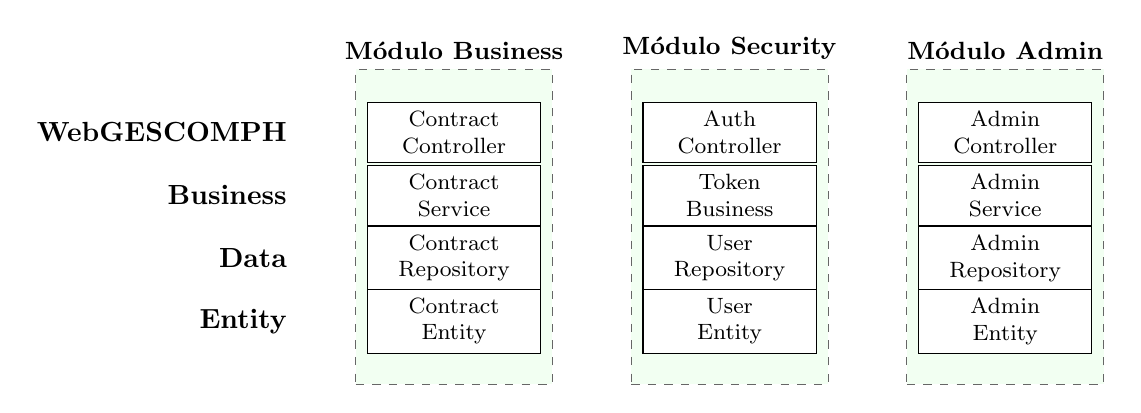
\begin{tikzpicture}[
    every node/.append style={font=\small},
    module/.style={rectangle, draw=black!60, dashed, fill=green!5, minimum width=2.5cm, minimum height=4cm, label=above:\textbf{#1}},
    layer/.style={rectangle, draw=black, fill=white, minimum width=2.2cm, minimum height=0.6cm, align=center, font=\footnotesize}
]
    % Módulo Business
    \node[module=Módulo Business] (modBusiness) at (0,0) {};
    \node[layer] at (0, 1.2) {Contract\\Controller};
    \node[layer] at (0, 0.4) {Contract\\Service};
    \node[layer] at (0, -0.4) {Contract\\Repository};
    \node[layer] at (0, -1.2) {Contract\\Entity};

    % Módulo Security
    \node[module=Módulo Security] (modSecurity) at (3.5,0) {};
    \node[layer] at (3.5, 1.2) {Auth\\Controller};
    \node[layer] at (3.5, 0.4) {Token\\Business};
    \node[layer] at (3.5, -0.4) {User\\Repository};
    \node[layer] at (3.5, -1.2) {User\\Entity};

    % Módulo Admin
    \node[module=Módulo Admin] (modAdmin) at (7,0) {};
    \node[layer] at (7, 1.2) {Admin\\Controller};
    \node[layer] at (7, 0.4) {Admin\\Service};
    \node[layer] at (7, -0.4) {Admin\\Repository};
    \node[layer] at (7, -1.2) {Admin\\Entity};

    % Etiquetas de capas laterales
    \node[anchor=east, font=\bfseries] at (-2, 1.2) {WebGESCOMPH};
    \node[anchor=east, font=\bfseries] at (-2, 0.4) {Business};
    \node[anchor=east, font=\bfseries] at (-2, -0.4) {Data};
    \node[anchor=east, font=\bfseries] at (-2, -1.2) {Entity};

\end{tikzpicture}
}
    \caption{Visualización de la Modularidad Vertical (Vertical Slicing). Cada módulo funcional atraviesa todas las capas arquitectónicas, facilitando la futura extracción a microservicios.}
    \label{fig:modularidad_vertical}
\end{figure}

Esta simetría, que también se observa en los módulos \texttt{AdministrationSystem}, \texttt{SecurityAuthentication} y \texttt{Locations}, reduce drásticamente la carga cognitiva del desarrollador. Si es necesario modificar la lógica de "Seguridad", el desarrollador sabe exactamente dónde buscar en cada proyecto (\texttt{SecurityAuthentication}). Esta organización mitiga la \textbf{Deuda Técnica Arquitectónica} identificada por \cite{architectural_debt_toledo}, facilitando el mantenimiento y, crucialmente, permitiendo que en el futuro un módulo entero pueda ser extraído a un microservicio independiente con un esfuerzo mínimo, tal como sugieren los patrones de migración de \cite{migration_monolith_mazzara}.

\subsection{Seguridad Transversal y Gestión de Identidad}

La seguridad no es un módulo aislado, sino un aspecto transversal (\textit{Cross-Cutting Concern}). La implementación utiliza \textbf{JWT (JSON Web Tokens)} para gestionar la identidad de manera "stateless". El componente \texttt{TokenBusiness.cs} en la capa de negocio genera tokens firmados que contienen los \textit{claims} (permisos) del usuario.

En la capa de presentación (\texttt{WebGESCOMPH}), un middleware personalizado intercepta cada petición HTTP, valida la firma criptográfica del token y establece el contexto del usuario antes de que la petición llegue al controlador. Este enfoque elimina la necesidad de sincronizar sesiones en el servidor, lo que permite que la API escale horizontalmente en entornos de nube sin problemas de afinidad, cumpliendo con las mejores prácticas de seguridad para sistemas distribuidos descritas por \cite{enhancing_security_patlolla}.

\subsection{Proyección Tecnológica y Trabajo Futuro}

Aunque la implementación actual establece una base sólida y funcional para GESCOMPH, el diseño modular se ha concebido para facilitar la incorporación progresiva de tecnologías emergentes. Reconociendo que el desarrollo de software es un proceso iterativo, se han identificado áreas clave para la evolución futura del sistema, alineadas con las tendencias académicas y de la industria:

\begin{itemize}
    \item \textbf{Automatización y DevOps:} Si bien la arquitectura actual soporta pruebas unitarias, el siguiente paso lógico es la integración de pipelines de CI/CD completos que incluyan pruebas de seguridad automatizadas, tal como proponen \cite{integrating_cybersecurity_manikyala}. Asimismo, se contempla la adopción de estrategias de \textit{Chaos Engineering} para poner a prueba la resiliencia del sistema ante fallos controlados, siguiendo las metodologías de \cite{chaos_engineering_nandigam}.
    
    \item \textbf{Seguridad Predictiva e IA:} Aprovechando la segregación de la lógica de negocio, se planea la futura integración de módulos de Inteligencia Artificial para la detección de anomalías en tiempo real. Referencias como \cite{predictive_cyber_resilience_konakanchi} sugieren que los microservicios (o módulos independientes) pueden autodefenderse mediante modelos predictivos, una capacidad que nuestra arquitectura modular podría adoptar sin reescribir el núcleo del sistema.
    
    \item \textbf{Evolución hacia Blockchain:} Para garantizar la inmutabilidad de los contratos públicos, se evalúa la posibilidad de integrar mecanismos de consenso basados en Blockchain en el módulo de seguridad, una dirección investigada por \cite{dynamic_adaptive_api_kaul} para marcos de seguridad adaptativos.
\end{itemize}

Esta hoja de ruta demuestra que la elección del Monolito Modular no es un punto final, sino una plataforma estratégica que permite a GESCOMPH evolucionar tecnológicamente sin comprometer su estabilidad operativa actual.
